% --- [ Performance ] ----------------------------------------------------------

\subsection{Performance}

The performance characteristics of the various components have been considered during every stage of the development process, but the initial prototypes have prioritized correctness and simplicity over performance. These prototypes have aimed at identifying suitable data structures and algorithms for the problems, through iterative redesigns and reimplementations. Once the major design decisions stabilized, production quality prototypes were being developed and thoroughly tested. To limit the risk of premature optimizations, micro-level performance work was intentionally postponed to the later stages of development.

Components with straight forward implementations (e.g. the LLVM IR library) have been profiled to identify performance bottle necks, as further described in section \ref{sec:profiling}. When estimating the time complexity of various subgraph isomorphism search algorithms however, algorithm research and the use of intuition proved far more valuable. One of the first throw-away prototypes provided a partial implementation of the subgraph isomorphism algorithm proposed by Ullman. After further research the prototype was eventually discarded as the Ullman algorithm had been proven to scale poorly for randomly connected graphs with more than 700 nodes \cite{iso_performance_comparison}. To put this into perspective, the \texttt{main} function of the c4\footnote{C in four functions: \url{https://github.com/rswier/c4}} compiler consists of 248 basic blocks. In other words, the CFG of the \texttt{main} function is a connected graph (every node is reachable from the entry node) with 248 nodes. This leaves a margin, for the number of basic blocks in functions, of less than an order of magnitude before the Ullman algorithm starts to perform poorly.

There exist several subgraph isomorphism algorithms which scale better than the Ullman algorithm for graphs with a large number of nodes; such as the VF2 algorithm for dense graphs and McKay's nauty algorithm for sparse graphs \cite{iso_performance_comparison,subgraph_isomorphism_algorithms}. In the case of the c4 compiler, the CFGs are sparse with $ 1.35 $ edges per node in average, which would favour the nauty algorithm.

% TODO: The time complexity is most certainly wrong. Reformulate the following paragraph and remove the reference to the time complexity.

The aformentioned subgraph isomorphism algorithms have been designed to support both connected and disconnected graphs, but the CFG are known to always be connected. By exploiting this property, a subgraph isomorphism search algorithm has been implemented which has a time complexity of $ \Theta{n \cdot m} $, where $ n $ is the number of nodes in the graph (i.e. the CFG) and $ m $ is the number of nodes in the subgraph (i.e. the graph representation of the high-level control flow primitive). Furthermore, $ m $ is known to be at most $ 4 $ for the currently supported high-level control flow primitives, which are presented in figure \ref{fig:graph_representations}.

In summary, profiling is great for optimizing the implementations of simple problems. Algorithm research, runtime complexity theory and intuition is essential for implementing performant solutions for complex problems. Furthermore, knowledge about specific properties of the problem may be exploited to design a performant algorithm.

% --- [ Subsubsections ] -------------------------------------------------------

% ~~~ [ Profiling ] ~~~~~~~~~~~~~~~~~~~~~~~~~~~~~~~~~~~~~~~~~~~~~~~~~~~~~~~~~~~~

\subsubsection{Profiling}
\label{sec:ver_profiling}

The initial implementation of the LLVM IR lexer (see section \ref{sec:impl_llvm_ir_library}) focused on correctness, and strived to be as simple and straight forward as possible. Once feature complete and thoroughly tested, the lexer was profiled for the first time and a major performance bottleneck was identified; as illustrated in figure \ref{fig:lexer_pprof}. When scanning letters, the \texttt{lexLetter} function used a hash map to check if the scanned letters were part of a keyword. As letters make up the majority of the characters in LLVM IR source files, this caused an extensive number of hash map iterations which accounted for roughly 70\% of the total execution time. To fix this issue, a benchmark test was implemented to measure the performance changes between the original and the updated version; as further described in section \ref{sec:ver_benchmarks}. At this stage, only CPU profiling has been utilized to identify performance bottlenecks. Future work may leverage memory profiling to further improve the performance of the decompilation components.

\begin{figure}[htbp]
	\begin{center}
		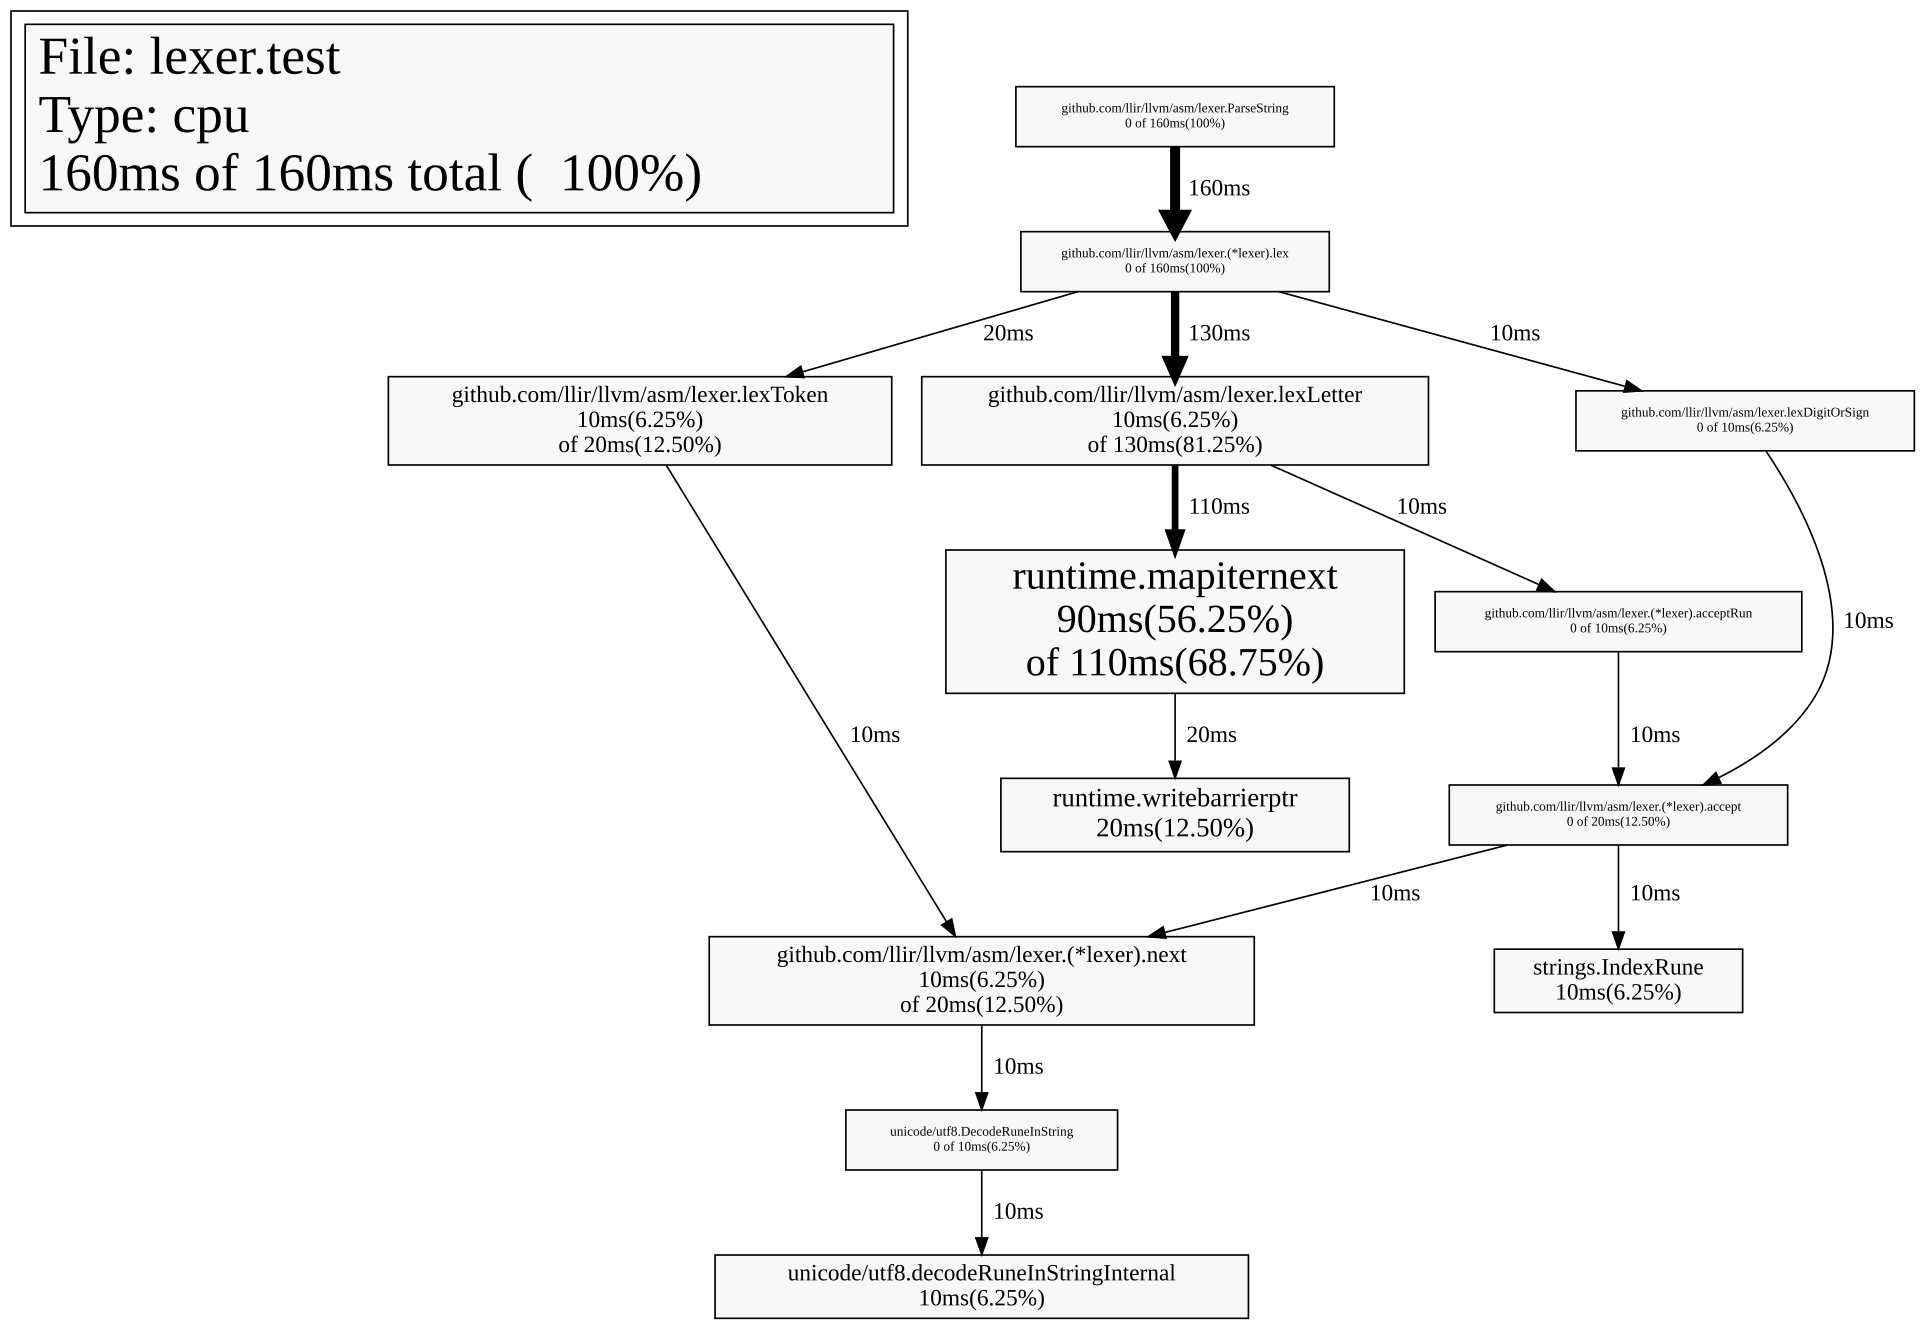
\includegraphics[width=\textwidth]{inc/8_ver/lexer_pprof.png}
		\caption{A major performance bottleneck was located when profiling the LLVM IR lexer for the first time. Roughly 70\% of the total execution time was spent doing hash map iterations (i.e. \texttt{runtime.mapiternext}).}
		\label{fig:lexer_pprof}
	\end{center}
\end{figure}

% ~~~ [ Benchmarks ] ~~~~~~~~~~~~~~~~~~~~~~~~~~~~~~~~~~~~~~~~~~~~~~~~~~~~~~~~~~~

\subsubsection{Benchmarks}
\label{sec:ver_benchmarks}

Benchmark tests were implemented to reliably measure any performance changes before trying to resolve performance issues. An updated version of the LLVM IR library used arrays instead of hash maps to identify keywords when scanning letters, which resolved the performance issue identified in section \ref{sec:ver_profiling}. The updated version of the LLVM IR lexer is roughly 3.6 times faster than the original version, as illustrated in figure \ref{fig:benchmark_delta}.

\begin{figure}[htbp]
	\begin{center}
		\begin{verbatim}
$ git checkout old; go test -bench=ParseString > old.txt
$ git checkout new; go test -bench=ParseString > new.txt
$ benchcmp old.txt new.txt
benchmark                old ns/op     new ns/op     delta
BenchmarkParseString     737625        204010        -72.34%
		\end{verbatim}
		\caption{Benchmark run time delta between the original and the optimized version of the LLVM IR lexer, as visualized by \texttt{benchcmp}\protect\footnotemark. The optimized version is roughly 3.6 times faster than the original vesion of the lexer.}
		\label{fig:benchmark_delta}
	\end{center}
\end{figure}
\footnotetext{Benchcmp displays performance changes between benchmarks: \url{https://golang.org/x/tools/cmd/benchcmp}}

